\chapter{Nástroj Node-RED}
\label{ch:nastroj-node-red}

V~této kapitole budou popsány základní principy nástroje Node-RED, vzhledem k~jeho funkci ve světě Internetu věcí, a
jeho důležité aspekty.
Node-RED je nástroj tvůrci popsaný jako \uv{Flow-based programming for the Internet of Things}, tedy nástroj založený na
programování na datovém toku určený pro IoT. Uživateli-programátorovi nabízí jednotlivé funkční bloky (či \emph{uzly}
dle kontextu),
jejichž vstupy a výstupy lze vzájemně propojovat a vytvářet tak síť jakožto celek s~požadovanými funkcemi.
V~roce 2013 jej představila společnost IBM v~rámci projektu JS Foundation pod licencí Apache 2.0. Nástroj vyžaduje
běhové prostředí Node.js, tedy je implementován v~programovacím jazyce Javascript, od čehož se odvíjí možnosti
jeho rozšiřování.

\begin{figure}
    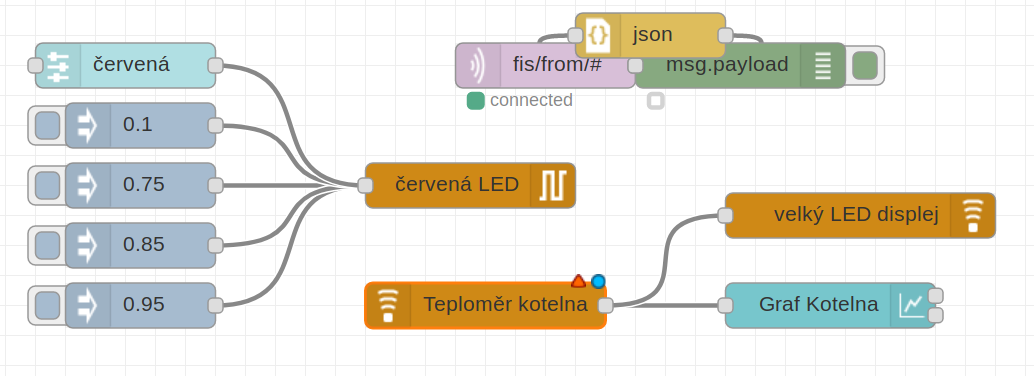
\includegraphics[width=\textwidth]{figures/node-red-example.png}
    \label{fig:node-red-example}
    \caption{Ukázka z~nástroje Node-RED -- vstupy a výstupy jednotlivých uzlů spojené pro vzájemnou komunikaci.
    V~levé části se nachází soustava bloků typu \uv{inject}, pomocí kterých lze manuálně odeslat zprávu do vlastního
    bloku ovládající periferii červené LED diody.
    Pravá spodní část patří měření teploty pomocí bloku teploměru, který data předává do grafu a na blok
    reprezentující displej.}
\end{figure}

\subsubsection{Programování datového toku}
Programovací paradigma založené na editaci datového toku bylo popsáno v~již v~dubnu roku 1974 vědcem Dennisem. Jeho
principem je programování pomocí vytváření datových spojů mezi funkčními bloky.
Ve své knize \uv{First Version of a Data Flow Procedure Language}~\cite{FirstVersionOfDataflow} popisuje sémantický
význam funkčních bloků propojených pomocí propojů, které zajištují vzájemnou komunikaci.

\section{Základní principy nástroje Node-RED}\label{sec:zakladni-principy-node-red}

Vnitřní architektura nástroje Node-RED je rozdělena na dva samostatné funkční části.
Z~pohledu samotného běhu je důležitější částí jádro provádějící veškeré datové operace nad samotným nadefinovaným
modelem, zodpovědné za spouštění jednotlivých uživatelských uzlů, jejich synchronizaci a vzájemnou distribuci dat.
Druhou částí je samotný vizuální editor, který je ve výchozím nastavení dostupný pomocí protokolu HTTP. Pomocí něj je
možné uživatelsky nastavovat jednotlivé uzly a vytvářet mezi nimi datové spoje.

Toto rozdělení nabízí možnost běhu sítě mimo samotný editor, a to především kvůli bezpečnostním a
výkonnostním důvodům -- každé \uv{flow} (množina entit funkčních uzlů a jejich propojení, dále jen
\emph{sít}\footnote{Pro \uv{flow} by se dal uvažovat taktéž překlad \uv{tok},
příp. přímo \uv{datový tok}, což ale příliš nekoresponduje s~praktickou stránkou věci -- \uv{síť} je reprezentativnější
pojmenování pro strukturu vytvářenou editorem nástroje Node-RED, i například vzhledem k~pojmenování Petriho sítí.}) je
schopen Node-RED serializovat do formátu JSON, tedy i ukládat či načítat do, resp. ze souborů, díky čemuž lze jednotlivé
sítě i snadno sdílet.

Mechanika samotných zpráv a jejich doručování je založena na několika základních premisách~\cite{NodeRedFlows}:
\begin{enumerate}
    \item Zprávy jsou obecně \emph{Javascript} hodnoty, standardně datového typu \ic{Object},
    tedy množiny dvojic \emph{klíč-hodnota}.
    \item Každý z~funkčních uzlů může vlastnit $0-N$ vstupních portů, stejně tak $0-M$ výstupních portů.
    \item Jednotlivé výstupy a vstupy lze propojovat, a to i vícenásobně, tedy více výstupů lze připojit na jeden vstup,
    stejně tak z~jednoho výstupu lze použít spojení do více vstupů.
    \item Zodpovědností uzlů je provedení definované funkce na základě přijaté zprávy nebo
    jiného externího vstupu.
    \item Zodpovědností sítě je distribuce zpráv mezi uzly a jejich asynchronní spouštění.
\end{enumerate}

Node-RED bez dalších rozšíření nabízí širokou základní sadu uzlů, mezi ty nejobecněji použitelné patří:

\begin{itemize}
    \item\emph{function} -- Blok vykonávající nakonfigurovaný uživatelský kód v~programovacím jazyce Javascript pro
    každou příchozí zprávu.
    \item\emph{inject} -- Interaktivní blok umožnující uživateli editoru zaslat konkrétní zprávu na výstup tohoto bloku
    přímo z~editoru (tedy internetového prohlížeče) -- vhodné především pro testování či manuální zasílání zpráv.
    \item\emph{debug} -- Blok poskytující logovací službu, dle jeho konfigurace jsou přijaté zprávy logovány do systémové konzole či do
    bočního panelu v~editoru -- vhodné pro testování a monitorování stavu sítě.
    \item\emph{switch} -- Blok starající se o~směrování zpráv v~síti -- na základně definovaných pravidel
    (shoda či porovnání hodnot, regulární výrazy) rozhodne, který z~výstupů bude použit pro další směrování zprávy.
    \item\emph{delay} -- Blok umožňující časové operace nad tokem zpráv skrz tento blok - dle konfigurace zprávy buď
    pouze zpožďuje o~konstantní hodnotu, nebo omezuje průtok (šířku pásma) za časovou jednotku.
    \item\emph{link} -- Blok, který je schopen zprávy exportovat do jiné sítě v~rámci jedné instance nástroje
    Node-RED -- vytváří jednosměrný tunel pro mezi-síťové směrování zpráv.
\end{itemize}

Pro bloky využívající externí služby nabízí Node-RED institut konfiguračních bloků.
Tyto bloky jsou pouze virtuální, v~síti se viditelně nevyskytují, ale je
s~jejich pomocí možné sdílet a znovupoužívat statickou konfiguraci v~dalších blocích.
Jedním takovým konfiguračním blokem je blok pro připojení k~brokeru MQTT, jehož konfigurační formulář je vyobrazen na
obrázku~\ref{fig:node-red-mqtt-out-conf:mqtt-broker})

\begin{figure}%
    \centering
    \subfloat[konfigurace výstupního MQTT bloku -- modře zvýrazněn vybraný broker MQTT]%
    {{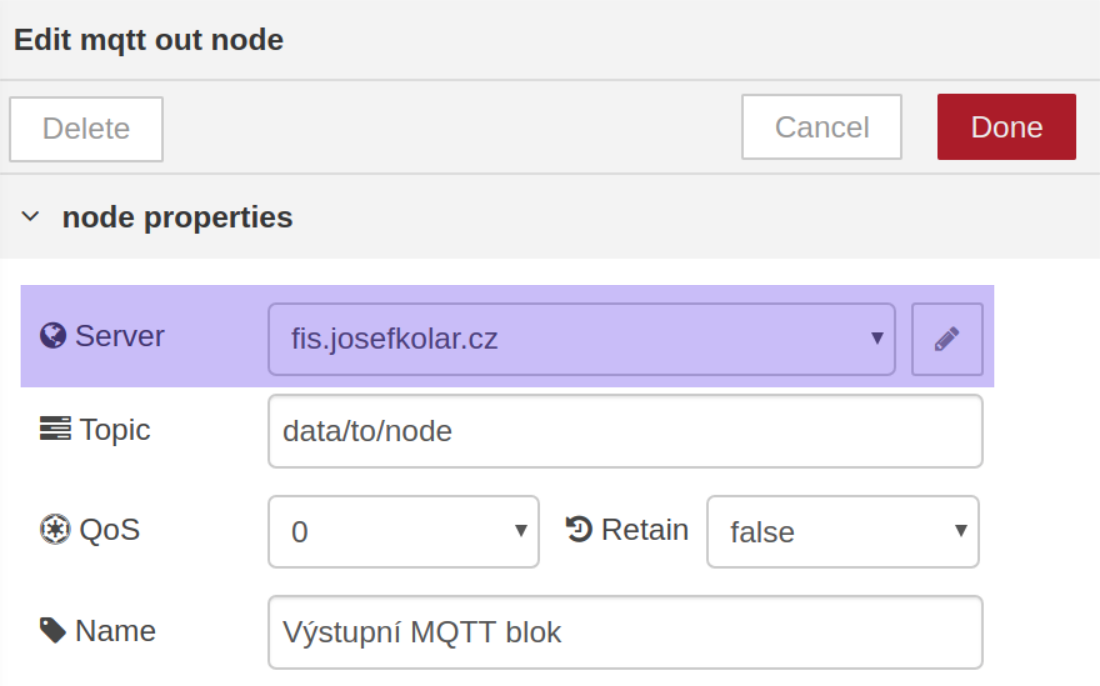
\includegraphics[valign=t,width=.49\textwidth]{figures/node-red-mqtt-out-conf.png}}%
    \label{fig:node-red-mqtt-out-conf:mqtt-out}}%
    \hfill
    \subfloat[konfigurace připojení k~brokeru MQTT -- konfigurační blok]%
    {{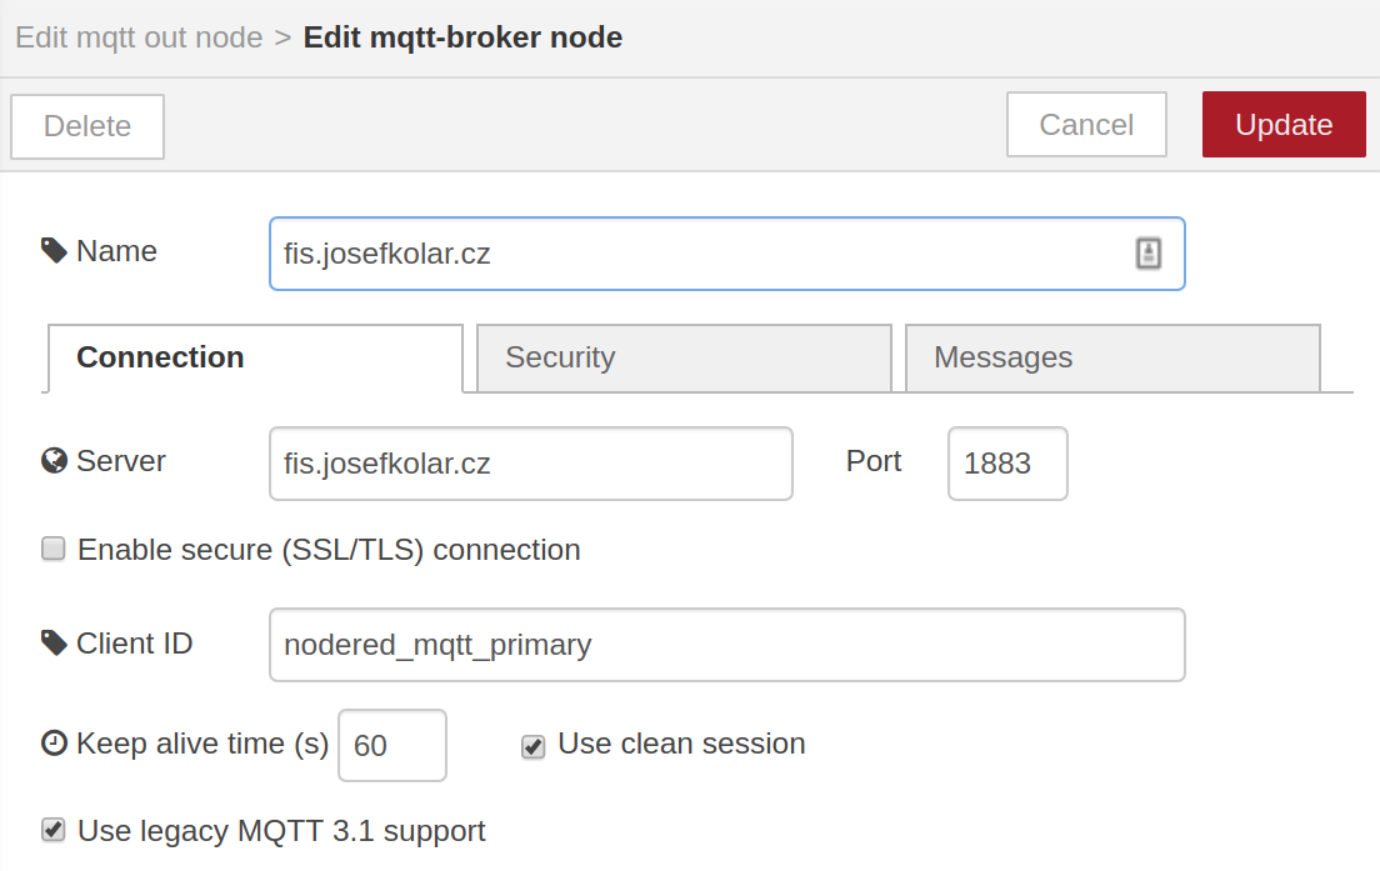
\includegraphics[valign=t,width=.49\textwidth]{figures/node-red-mqtt-broker-conf.png}%
    \label{fig:node-red-mqtt-out-conf:mqtt-broker}}}%
    %
    \caption{%
    Konfigurace výstupního MQTT bloku zahrnuje nastavení celého bloku (výstupní kanál, QoS, příznak \uv{retain}
    či pojmenování samotného bloku) a nastavení samotného MQTT připojení (cílový server, identifikace klienta či
    autentizační údaje)
    }%
    \label{fig:node-red-mqtt-out-conf}
    %
\end{figure}


\section{Rozšíření pomocí vlastních modulů}\label{sec:node-red-rozsireni}

Nástroj Node-RED mj. díky své otevřenosti nabízí rozšiřování pomocí vlastních bloků s~vlastním chováním.
Při startu tento nástroj proskenuje jmenný prostor nainstalovaných knihoven a do užšího výběru vybere
knihovny s~názvem začínajícím na {\ic{node-red-contrib-}} -- tento prefix značí, že knihovna může obsahovat
rozšiřující bloky. % mbox hack to no break in the middle
Standardem v~ekosystému jazyka Javascript je soubor \texttt{package.json} obsahující metainformace o~konkrétním
balíčku (knihovně) -- v~tomto souboru vyhledává Node-RED klíč \texttt{node-red} a následně \texttt{nodes}.

Balíček takto exportuje uzly, které jsou zařazeny do galerie všech dostupných uzlů -- reprezentaci v~galerii zajišťuje
soubor se zdrojovým kódem v~jazyce HTML.
V~tomto souboru je pro uzel definován název, nápověda či ikona, ale především počet vstupů a výstupů a vlastní
konfigurační parametry, které se následně zobrazují jako nastavitelné přímo v~editoru -- kromě standardních vstupů
pro řetězce se může jednat o~výběr z~výčtu, výběr barvy či výběr konfiguračního bloku popsaného výše
(obrázek~\ref{fig:node-red-mqtt-out-conf:mqtt-out} zachycuje možnosti definice parametrů ve výstupním bloku MQTT).

Druhým souborem je soubor v~jazyce Javascript popisující chování samotného uzlu -- zde jsou definovány reakce na
přicházející zprávy (implementace zpracovávající příchozí zprávy), ale také připojení na služby dalších stran.
Standardním obsahem tohoto souboru je funkce, která ve svém těle registruje konkrétní blok do centrálního registru
bloků a následně i implementace tohoto bloku.
Z~editoru jsou zde dostupné nakonfigurované parametry (v~parametru funkce), které mohou být následně použity pro
úpravu chování bloku.
Ve zdrojovém kódu~\ref{code:node-red-custom-block} se nachází ukázka implementace jednoduchého rozšiřujícího bloku --
v~bloku hlavní funkce je navázána funkce obsluhující událost typu \ic{\'input\'}.
Na základě této události je zpracována příchozí zpráva a výsledek je opět dál odeslán jako zpráva datového typu
\ic{Object}.

% @formatter:off
\begin{code}[%
    caption={Ukázka implementace vlastního rozšiřujícího bloku do nástroje Node-RED -- uzel s~jedním vstupem a
výstupem, jehož funkcí je určení délky příchozí zprávy (řetězce).
\emph{Implementace pro jednoduchost neobsahuje kontrolu datových typů či práci s~konfiguračními parametry uzlu.}},
    label=code:node-red-custom-block,
    language=Javascript
]
function StringLengthNode(config) {
    RED.nodes.createNode(this, config);
    var node = this;
    node.on('input', function(msg) {
        msg.payload = msg.payload.length;
        node.send(msg);
    });
}
RED.nodes.registerType("string-length", StringLengthNode);
\end{code}
% @formatter:on

\section{Node-RED Dashboard}\label{sec:node-red-dashboard}

\begin{figure}[th]
    \centering
    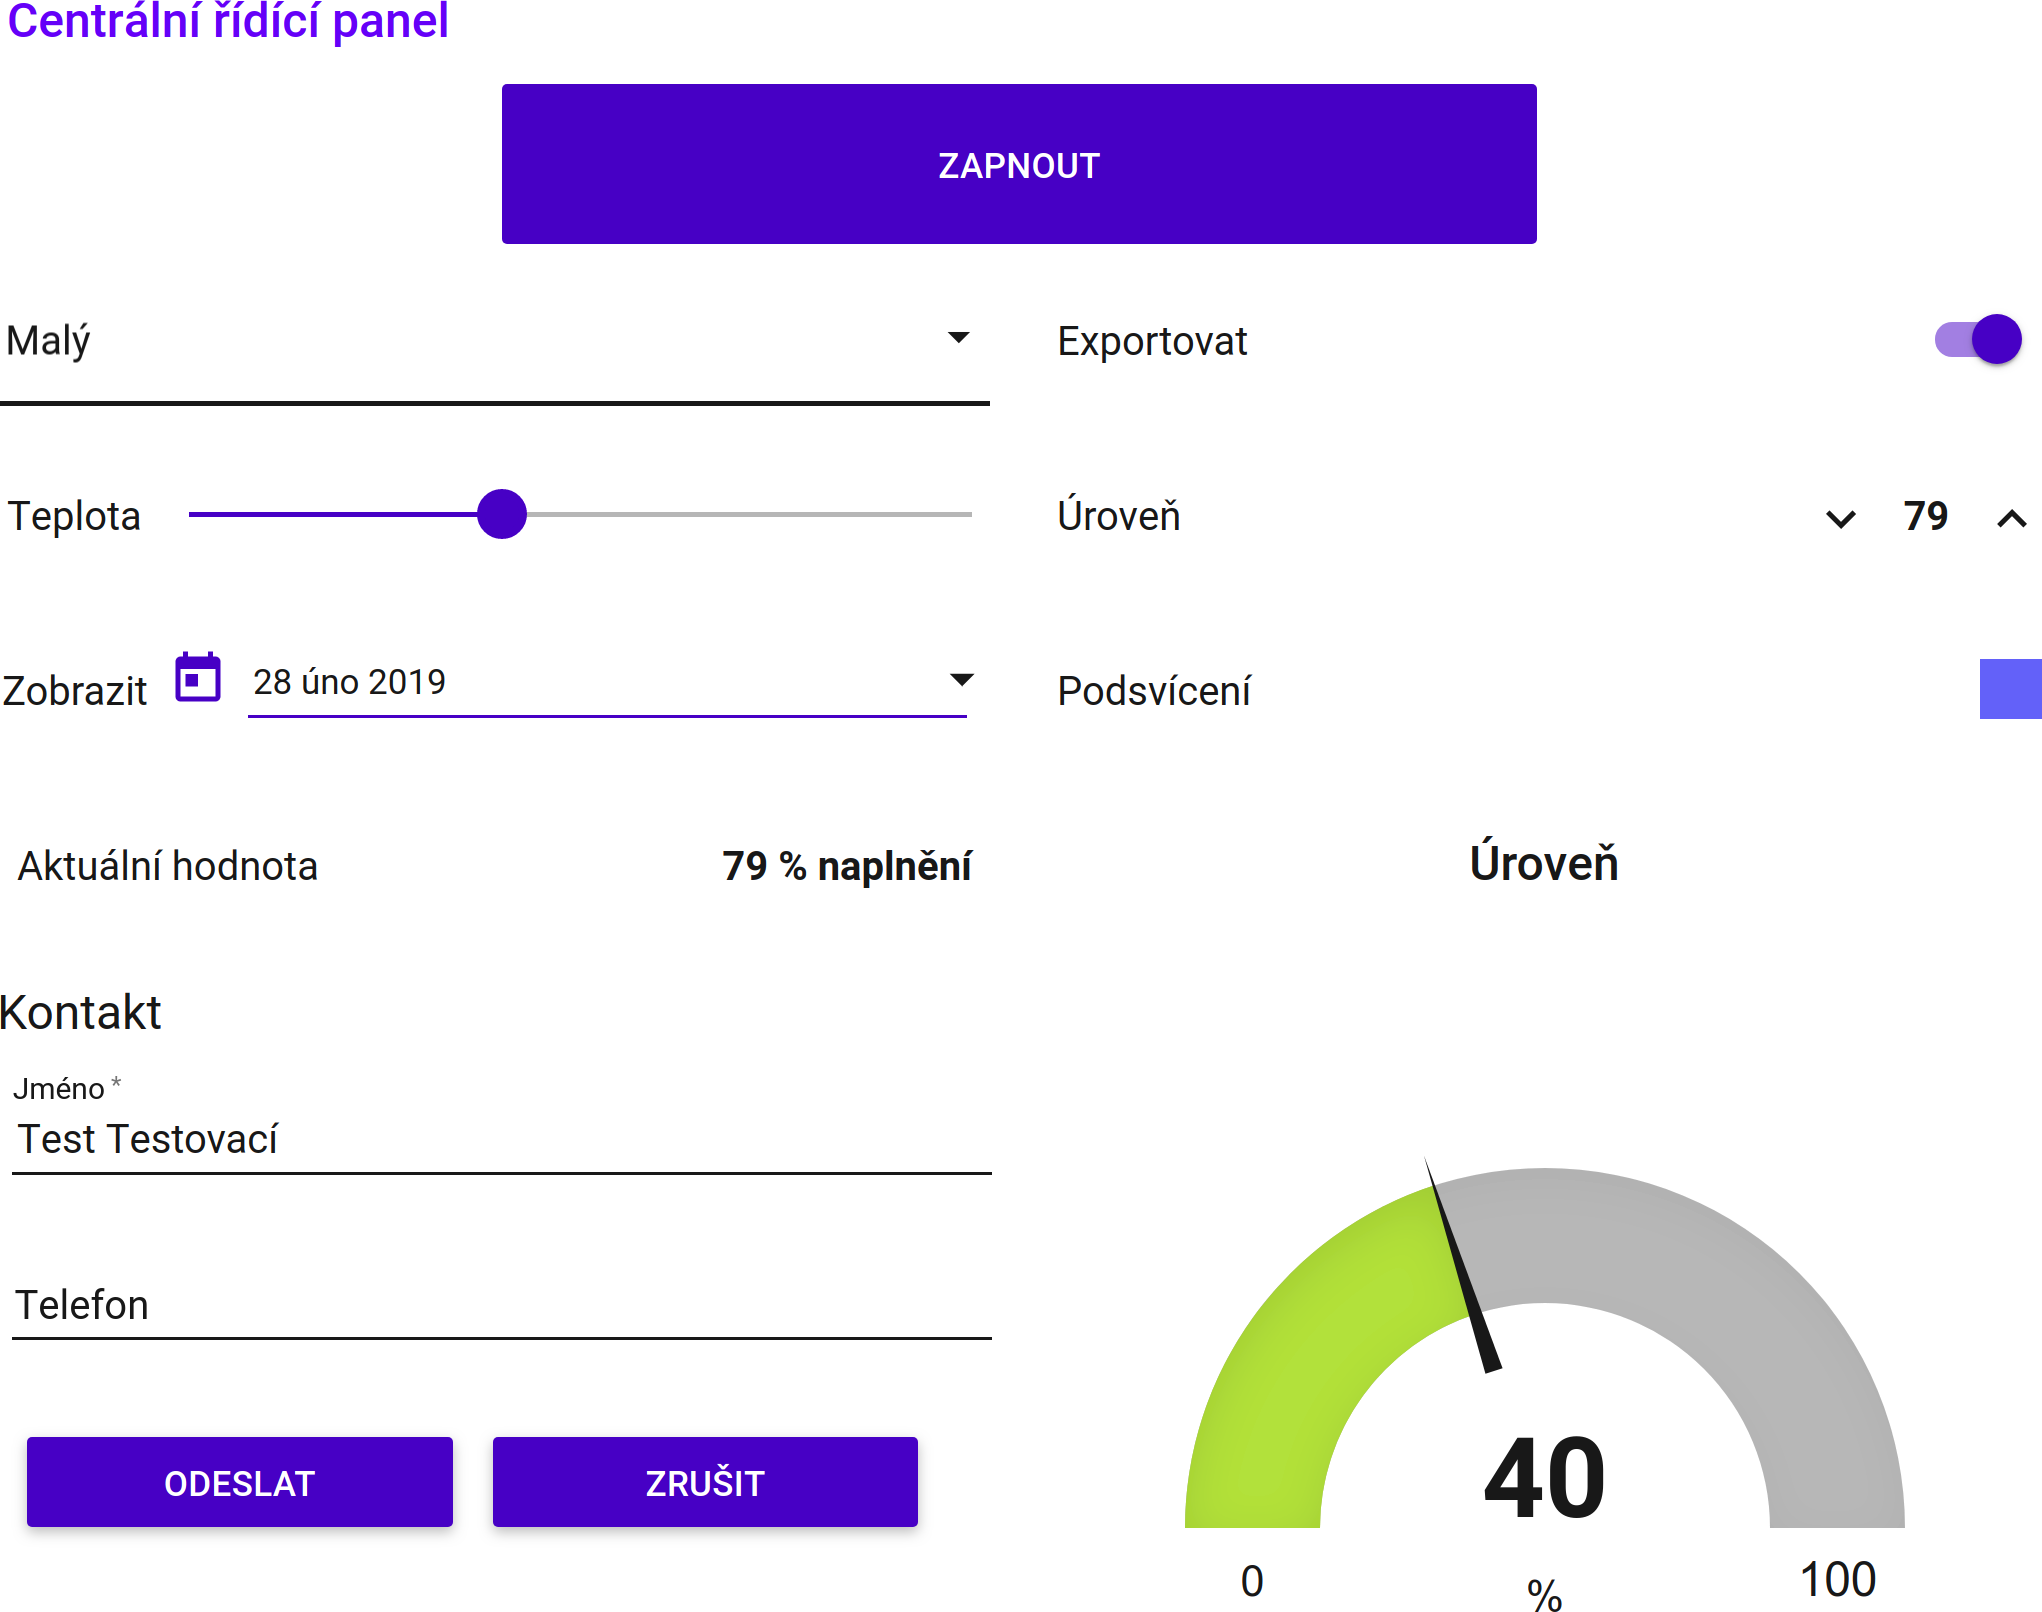
\includegraphics[width=\textwidth]{figures/node-red-dashboard.png}
    \caption{Ukázka uživatelského rozhraní postaveného pomocí balíčku \texttt{node-red-dashboard} -- možnosti sahají
    od standardních prvků typu tlačítka, textového vstupu, formuláře či checkboxu, přes dynamické textové výstupy,
    nastavení barvy a posuvníky až ke komponentám typu výstupní grafické výstupní škály či výběru data z~kalendáře.}
    \label{fig:node-red-dashboard}
\end{figure}

Díky otevřenosti ekosystému nástroje Node-RED vznikl populární rozšiřující balíček s~názvem
\texttt{node-red-dashboard}.
Tento balíček nabízí tvůrcům sítí zařadit i uživatelské rozhraní zahrnující dynamické
popisky, grafy, tlačítka a další akční a informační členy.
Definice tohoto rozhraní je založena na použití standardních funkčních bloků sítě, vstupní zprávy reflektuje nástroj
v~uživatelském rozhraní, naopak uživatelská interakce je reflektována výstupními zprávami z~bloků rozhraní.
Kromě definice samotných bloků lze další vlastnosti rozhraní konfigurovat v~přídavném postranním panelu v~editoru --
rozšíření definuje rozřazení do záložek, skupin, jejich vzájemné pozicování, pořadí a vzhled.
Ukázka možností rozhraní postaveného pomocí tohoto balíčku je zobrazena na obrázku~\ref{fig:node-red-dashboard}.

Z~pohledu sítě disponují bloky z~tohoto balíčku standardními vlastnostmi -- vstupy z~uživatelského rozhraní jsou
reflektovány pomocí výstupních zprávů bloků s~informacemi o~akci či změně vstupu, výstupní procedura z~hlediska sítě
je obdobná, bloky tohoto rozhraní jsou výstupními bloky sítě a balíček zajistí přenos informace ze sítě směrem do
uživatelského rozhraní.

